\documentclass{article}
\usepackage{picinpar,graphicx}
\graphicspath{{/home/li/图片/}}
\usepackage{multicol}
\usepackage{lscape}
\usepackage{cite}
\author{Qingyun Li}
\date{May 22, 2018}
\title{Fog and Smog}
\begin{document}
\maketitle
 \par As we all know, fog is a natural weather phenomenon. Especially recent yeays, due to the distruction of the   environment, this phenomenon is more and more serious. The buildings is higher and the air isn't free, all this reasons lead to the formation of the fog. And our common life has been effected seriously. 
 \par Fog consists of visible cloud water droplets or ice crystals suspended in the air at or near the Earth's surface\cite{gultepe2008fog}. So fog can be considered a type of low-lying cloud and is heavily influenced by nearby bodies of water, topography, and wind conditions.
 \par Next, the concentration level of fog will be discussed, we can learn it explicitly at the table 1.
\begin{table}[htbp]
\centering
\caption{Concentration level of fog}
\begin{tabular}{c|c}
\hline
Level & Horizontal Visibility Distence \\
\hline
mist & 1000-10000 \\
fog & 500-1000 \\
heavy fog & 200-500 \\
smoke fog & 50-200 \\
strong fog & <50 \\
\hline 
\end{tabular} 
\end{table}
 \par Given that the air pollution has been unprecedentedly severe in recent years, "smog" is more and more widly mentioned by everyone. This word is consist of two words, smoke and fog. We can learn it clearly from these words. Smog is different from fog, we can seen it at Fig.~\ref{differnce}, and it's a type of air pollution derived from vehicular emission from internal combustion engines and industrial fumes that react inthe atmosphere with sunlight to form secondary pollutants that also combine with the primary emissions to form photochemical smog.
 \begin{figure}[htbp]
\begin{minipage}{1\linewidth}
\centering{}
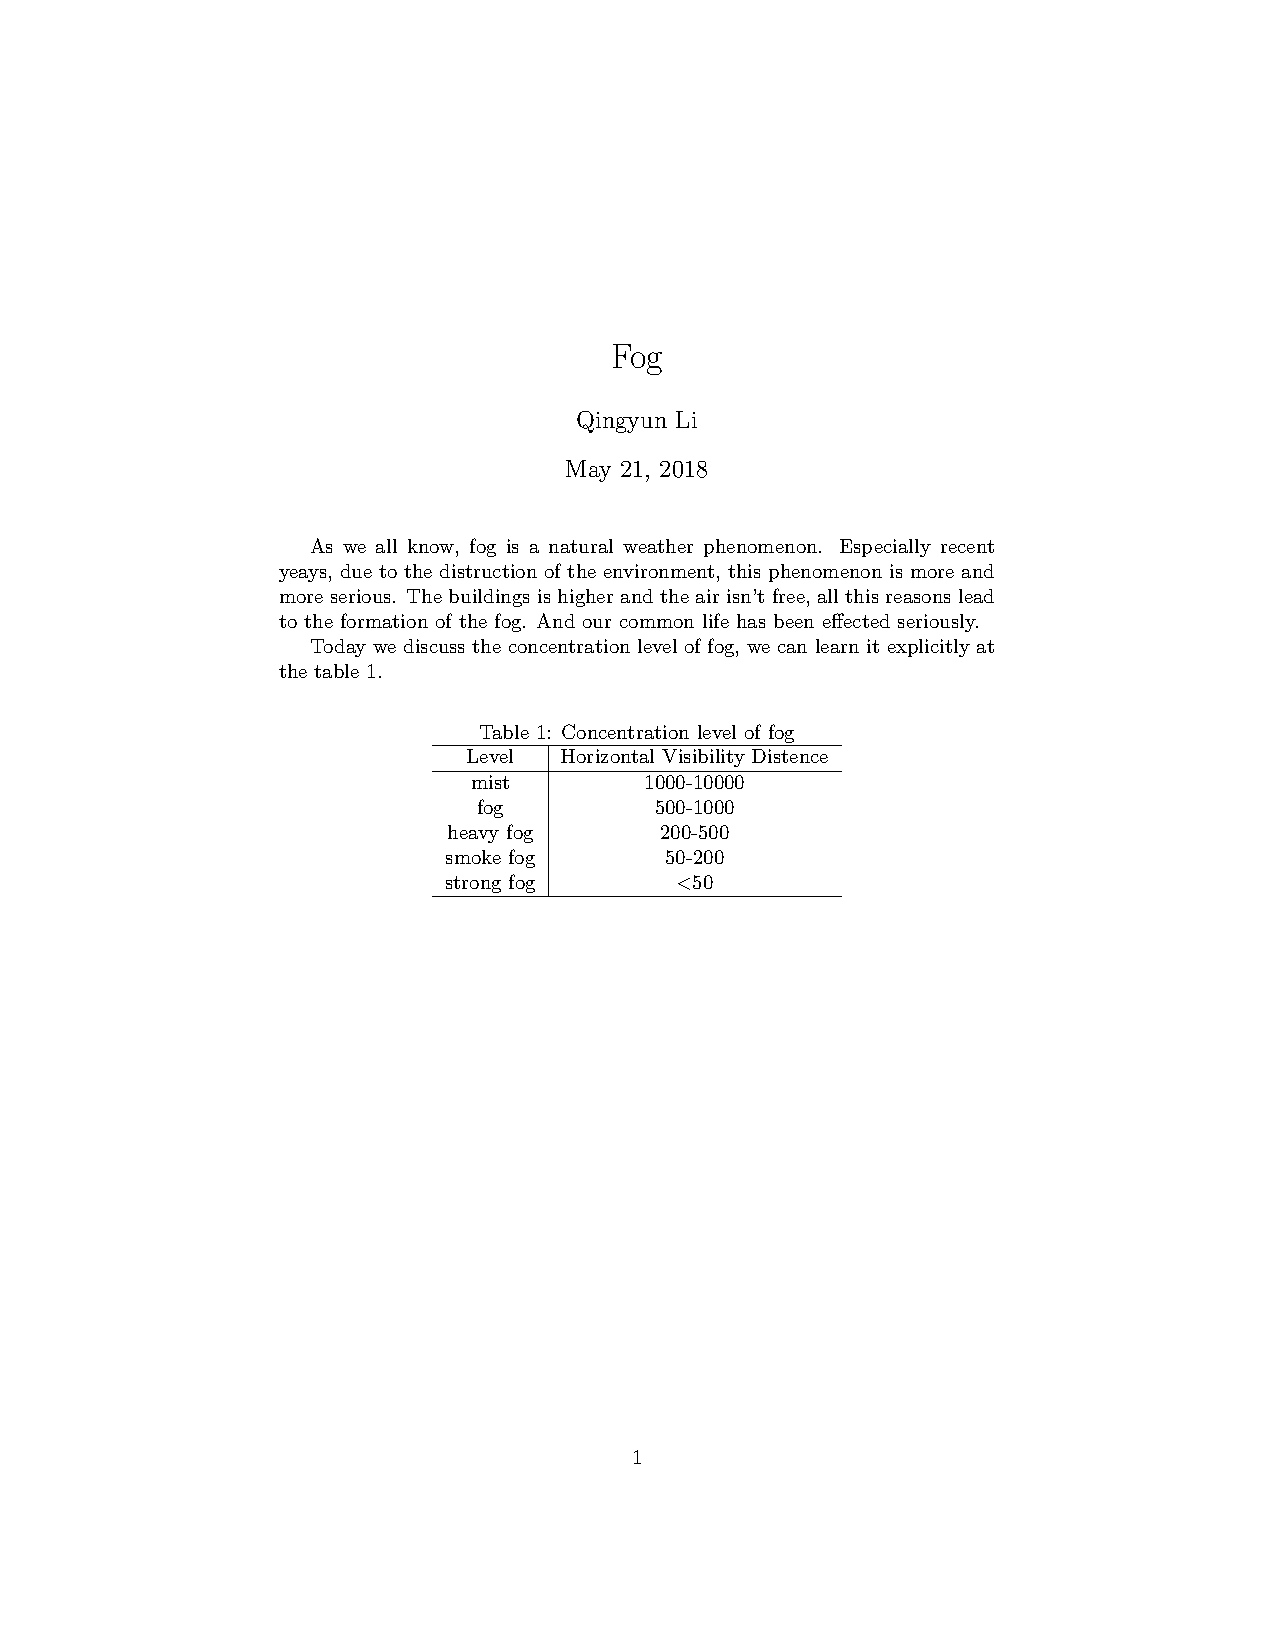
\includegraphics[width=0.7\linewidth]{Fog.jpeg}\\
\caption{The difference of the fog and smog}\label{differnce}
\end{minipage}
\end{figure}
\bibliographystyle{plain}
\bibliography{single}
\end{document}